\section{Background}
The section gives the necessary insights about sparse linear algebra to more clearly show the context of the work. Further, it discusses fusion, challenges and outlines the proposed solution. 

% standard, it's existing implementations, and expected optimizations as well as performance issues. Further the section surveys hardware implementations, techniques of software and hardware co-design, and justifies design choices made.
\subsection{GraphBLAS}\label{graphblas}
\emph{GraphBLAS} is a C API specification that standardizes sparse linear algebra building blocks initially for graph computations but is nevertheless applicable in other areas. It translates mathematical specifications to API that could be efficiently implemented in hardware or software. Also, it is the only such specification and was completed by researchers from the field of high-performance graph algorithms based on sparse linear algebra. The specification further gives the means for interoperation with vertex-centric libraries, which potentially makes it a crucial component in the future ecosystem of big graphs~\cite{sakr2020future}. A list of operations (not exhaustive, though) provided by the standard could be seen in table~\ref{tab:table_blass}, where $C\langle M \rangle$ stands for masking, i.e., taking a subset of elements that satisfies the mask or its complement. These are sufficient to express a lot of algorithms, e.g., \emph{PageRank}, \emph{Breadth-First-Search}, \emph{Sparse Deep Neural Network Graph Challenge}~\cite{SparseDNN}. Notably, each operation is parameterizable by a semiring, which is the key to expressivity. 

\begin{table}[b]
    \centering
    \begin{tabular}{ |c|c|c|c| } 
\hline
\rowcolor{LightBlue}
Function & Description & Notation \\
\hline
\texttt{GrB\_mxm} & matrix-matrix mult. & $C \langle M \rangle = AB$ \\ 
\texttt{GrB\_eWiseMult} & element-wise, set union &
$C\langle M \rangle = A \otimes B$\\ 
\texttt{GrB\_eWiseAdd} & element-wise, set-intersection  & $C \langle M \rangle = A \oplus B$ \\
\texttt{GrB\_apply} & apply unary op. & $C\langle M \rangle = f(A)$\\
\hline
\end{tabular}
    \caption{Some of the GraphBLAS operations}
    \label{tab:table_blass}
\end{table}


% A motivating, but not complete, example, illustrating the need for some of the building blocks could be seen in~\ref{listing:bfs}.

% \begin{listing}[h]
% \caption{Breadth-first search example}
% \label{listing:bfs}
% \centering

% \begin{minted}[linenos]{python}
% #Sparse algebra BFS:
% #times: if (A[i,j] != 0) A[i,j] × q(k) = k
% #       else 0
% #plus : any(x,y) = x or y randomly

% q = [source]; 
% parent = [0 for i in range(n)]; 
% parent[source] = source;

% while (q not empty)
%     #masked matrix vector multiplication
%     q<¬parent> = A*q #mask could be inverted
%     #masked assignment
%     parent<q> = q
% \end{minted}
% \end{listing}

% The example performs breadth-first graph traversal using matrix-vector multiplication over a semiring. An operation could be parameterized by a \emph{mask}, specifying what exactly elements are of a particular interest: in case of a masked matrix-vector multiplication only masked elements are non-zero. Masked operations are essentially the operations followed by element-wise multiplication with mask matrix, thus element-wise operations are also a part of the standard. Notably, the multiplication operation of the semiring from the example returns the index of the element in the vector, while still performing graph traversal~\cite{GAILLA}, and the plus operation could nondeterministically return any of its parameters. This allows to keep track of not only visited vertices but also of their parents, while masking prevents already visited vertices from being visited again.

These operations are often chained in such a way that makes fusion possible. Consider, for example, an excerpt from Luby's maximal independent set algorithm~\cite{SuiteSparseOnly} in listing~\ref{listing:fusion} depicted in pseudo-Haskell with mutable variables. It shows a sequence of element-wise additions which could be fused to eliminate the construction of a \mintinline{Haskell}{new_members} matrix in the middle. The result of such fusion depends on the implementation of \mintinline{Haskell}{GrB_eWiseAdd} and hence is not shown.

\begin{listing}
\centering
\caption{Excerpt from Luby’s maximal independent set algorithm implementation}
\label{listing:fusion}
\begin{minted}[fontsize=\small]{Haskell}

-- select node if its probability is > than all its active neighbors
let new_members = prob `GrB_eWiseAdd GrB_GT_FP64_Semiring` neighbor_max
-- add new members to independent set.
    iset = iset `GrB_eWiseAdd GrB_LOR_Semiring` new_members

\end{minted}


% GB_PUBLIC
% GrB_Info GrB_Matrix_apply           // C<Mask> = accum (C, op(A)) or op(A')
% (
%     GrB_Matrix C,                   // input/output matrix for results
%     const GrB_Matrix Mask,          // optional mask for C, unused if NULL
%     const GrB_BinaryOp accum,       // optional accum for Z=accum(C,T)
%     const GrB_UnaryOp op,           // operator to apply to the entries
%     const GrB_Matrix A,             // first input:  matrix A
%     const GrB_Descriptor desc       // descriptor for C, mask, and A
% ) ;

\end{listing}

\subsection{Fusion}

The formal definition of fusion is not obvious to give, and thus some intuitive understanding is assumed. Fusion optimization often stands for the removal of something intermediate, i.e., something which is first constructed and then deconstructed. These could be arrays for imperative programs, lists for functional programs, and whole kernels in the case of a GPU accelerated linear algebra library (kernel launch overhead is mitigated by gluing kernels into one). This section will give a brief overview of what is assumed by fusion in some systems and outline their implementation details. Note that only automatic fusion will be considered since the easy solution is to provide enough already fused primitives, but the approach has limited flexibility and high development costs.

% here we go
% imperative things with affine transformations
% Julia, some ad-hoc stuff
% XLA
% Futhark
% Stream fusion
% And finally distillation
% Producer consumer

In \textit{imperative languages}, fusion is often associated with gluing several loops into one. It may increase the locality and reduce the required memory consumption. The procedure often relies on polyhedral and affine analysis techniques and is infeasible if the loops exhibit non-affine indexing, which is just the case for sparse data structures. 

In \textit{functional languages}, we mainly deal with functions, and hence fusion in its simplest form is function composition, which is implemented as a term rewriting pass, e.g., \mintinline{text}{map f . map g == map (f . g)}. However, functions are less performant in representing data than, e.g., arrays, and some state-of-the-art solutions exist that provide fusion for high-order array operations in functional languages~\cite{Futhark}. But they also fail to fuse across index arithmetic which arises in sparse data structures. There was an attempt to implement sparse matrix e-wise addition in functional array programming language~\cite{Futhark}, but indexing appeared to be hard to fuse\footnote{Implementation is available here: \url{https://github.com/Tiltedprogrammer/impala-sparse/blob/master/futhark/sparse.fut} (online; accessed: 2022-06-07)}. 

Furthermore, rewrite rules are domain-specific. They are tightly coupled with, e.g., arrays or matrices where one could use distributive law to perform some kind of fusion. But, in sparse applications, it is often the case that we do not have any special properties like associativity and commutativity, e.g., in the case of context-free graph querying. However, it is worth noticing that such rewrite rules are very powerful when combined with staged compilation~\cite{stagedLinAlg}. Such rules also form the basis for a widely addressed area of \textit{stream fusion}~\cite{StreamFus}; however sparse matrices impose a particular structure and thus are not stream-like, and rules require to express programs with certain combinators.

In Tensorflow and its XLA compiler~\cite{TensorFlowXLA} a machine learning model is represented with a dataflow graph, in which tensors flow through the edges and nodes represent some operations. The goal of the compiler is to identify and offload some parts of such a graph to, e.g., GPU, and perform corresponding code generation. Fusion is performed on that graph level, either by duplicating producers for each consumer or fusing outputs of several operations. The approach works under the restrictions that the kernels comply with similar memory access and iteration patterns, which is hard to guarantee in sparse applications.  

Another approach to removing intermediate data structures in functional programs is \textit{distillation}~\cite{distillation}. It is a generalization of supercompilation~\cite{supercompilation}, and briefly, its goal is to represent all possible execution paths of a program with a finite process graph. Such a process graph is built by performing normal order reduction on terms, and the fusion effect is achieved by performing a transitive closure of such a graph. On top of that, distillation is able to provide superlinear programs speedup, perform specialization, and make other optimizations available by propagating positive information.

% \emph{Direction-based} optimization is in charge of either deciding to use sparse-vector or dense-vector operations for  matrix-vector multiplication. The current frontier during a graph traversal could grow while the mask of yet not-visited vertices becomes small, so it becomes more profitable to utilize masked dense operations instead of sparse-matrix sparse-vector operations.

% \emph{Load-balancing} optimization chooses the most suitable distribution among the workers (e.g. threads) depending on the sparsity of the operands. Or schedules the operands in a way to save computations, e.g. first merge two small arrays instead of a small and a large array in order to not extend a large array overhead throughout all the computation.

% \emph{Mask fusion}. Ahead-of-time masking could reduce the number of memory accesses in case of matrix-vector multiplication and prevent memory blow-up in case of matrix-matrix multiplication: the multiplication of two sparse matrices could produce an order of magnitude
% more non-zeroes in the output matrix compared with the two input matrices, hence the mask could limit the output number of non-zeroes, thus preventing out-of-memory errors. In order to achieve such a behavior, a mask should be fused (i.e. transformed in a single operation) with the corresponding operation for the operation to perform computations only for the elements in the mask. The effect of masking in case of sparse matrix-dense vector multiplication could be seen in figure~\ref{fig:fusion}. Ahead-of-time masking reduces the number of memory accesses from 8 to 3. Vectors are usually stored both in sparse and dense formats, hence masking could always be performed making sparse matrix-dense vector multiplication faster than sparse matrix-sparse vector multiplication in virtue of implementation details.

% \emph{Kernel fusion}. Mask fusion is a special case of kernel fusion. Kernel fusion is responsible for fusing arbitrary operations. In the case of loop-based programming fusion simply stands for joining several loops into one to increase memory locality and reduce the number of required iterations. It is a crucial technique in dense applications and is usually followed by a stage of \emph{polyhedral analysis}. This is extensively exploited in frameworks like TensorFlow and its XLA compiler~\cite{TensorFlowXLA}. 

% Some general-purpose solutions exists that support fusion, e.g., \cite{Futhark} which are based on map/reduce semantics. But in order to support sparse operations they should be able to fuse across index arithmetic, which is not the case. Thus a domain-specific language is needed designed with inherent support for indexing fusion. A motivating example for general fusion could be seen in listing~\ref{listing:fusion}, which is a snippet (simplified for demonstration) from Luby’s maximal independent set algorithm implementation~\cite{SuiteSparseOnly}. As could be seen it is a series of element-wise (e-wise for short) matrix additions: two consecutive element-wise operations could be fused, so \texttt{new\_members} matrix creation and further iteration are reduced. 



% \begin{minted}[escapeinside=||]{haskell}
% map f (map g list) |$\equiv$| map (f |$\circ$| g) list 
% \end{minted}


% \begin{listing}
% \centering
% \caption{Kernel fusion example}
% \label{listing:2}
% \begin{minted}{python}
% #Fusing together '+', '-', and masking
% #prevents two intermediate matrices allocation

% C<mask> = A + C - B
% \end{minted}
% \end{listing}

% \emph{Specialization}. Generally, it is a program transformation optimization~\cite{jones} that exploits the knowledge about some of the operation parameters, hence it could optimize those parts of the operation that depend on the known pieces of information. In the case of \emph{NVIDIA CUDA}\footnote{GPU programming architecture, used in~\cite{yang2020graphblast}.} specialization assigns a specialized computation per a warp\footnote{A group of threads that form a single unit of execution.}, since warps could be executed independently. This technique is well-described, e.g., in~\cite{CUDADMA}. An example of such optimization could be a matrix-vector multiplication in some cycle where the vector remains unchanged. Hence, the vector could be embedded in the operation itself avoiding vector-specific overheads, e.g, allocation or data transfer back-and-forth from host to device. Matrix-vector multiplication is essentially a linear combination of columns where each column has a corresponding coefficient from the vector. Thus, each warp could multiply it's assigned column by the \texttt{warp\_id's} element of the vector, which could be embedded in the code of the warp itself. Such embedding is generally a huge \texttt{warp\_id} \texttt{switch} statement, which incurs almost no overhead in the case of CUDA. But generally specialization is applicable only at the level of warps in CUDA and suffers from thread divergence in other scenarios. Thus a hardware accelerator with another hierarchy of workers could be a better fit taking in mind the specialization.

% what about it?
% \emph{Polyhedral compilation} \texttt{TBD}


\subsection{Challenges}\label{sec:challenges}
Despite the overall achieved performance of GraphBLAS implementations, there are inevitable challenges both for the hardware running sparse algorithms and for the software performing optimizations.

For the former, both CPUs and GPUs remain underutilized when executing sparse operations due to high cache-miss rates and limited communication between processors~\cite{Song_2016}. Sparse algorithms are inherently memory-bound, resulting in poor GFLOPs number compared to peak GFLOPs theoretically available on modern devices, namely less than $0.2\%$ of theoretical performance is achieved as reported in~\cite{leskovec2016snap, Florida}. For example, the pipeline of sparse matrix-matrix multiplication consists of several kernels that greatly vary in performance and resource utilization. For the case of a GPU implementation\footnote{Using cuSPARSE library and roadNet-CA graph.} the performance analysis is illustrated in figure~\ref{fig:SMperf}. Each kernel utilizes SM (Streaming multiprocessor) differently, where percentage means the number of cycles the SM is not idle. It is also worth noting that the utilization of floating-point units is still about 0\% for all the kernels. Also as it could be seen from the kernels' runtime, the \emph{reduce} kernel (the one that actually performs the operations, e.g., addition and multiplication) takes about 2\% of the time, while memory operations take the whole half of it. It means that full GPU power is needed only in 2\% of the pipeline time. 

% available power of GPU resources is idle (the runtime considers also all the overheads, e.g., memory transferring).

\begin{figure}
\begin{minipage}{0.45\textwidth}
    \centering
    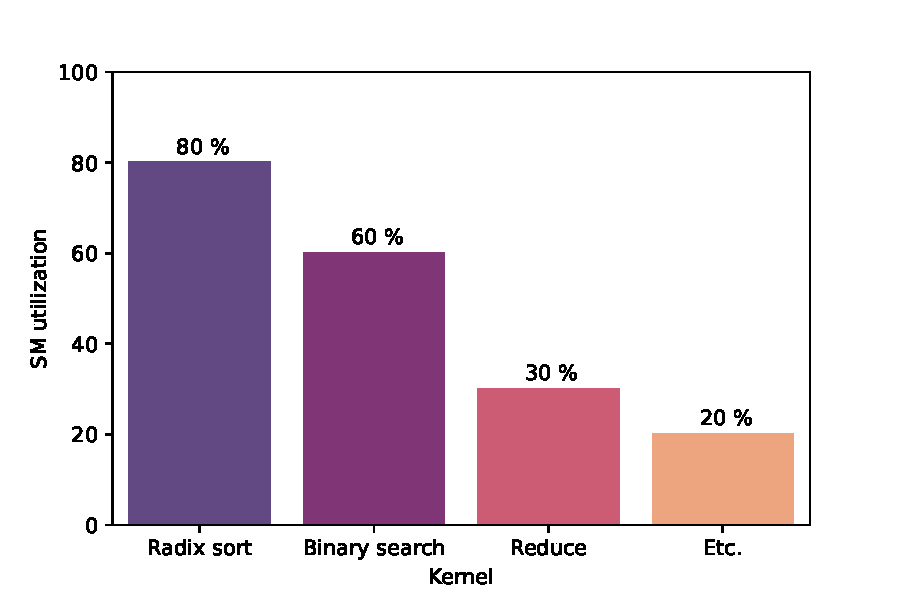
\includegraphics[width=\linewidth]{figures/fig_2_bar.pdf}
\end{minipage}
\hfill
\begin{minipage}{0.45\textwidth}
    \centering
    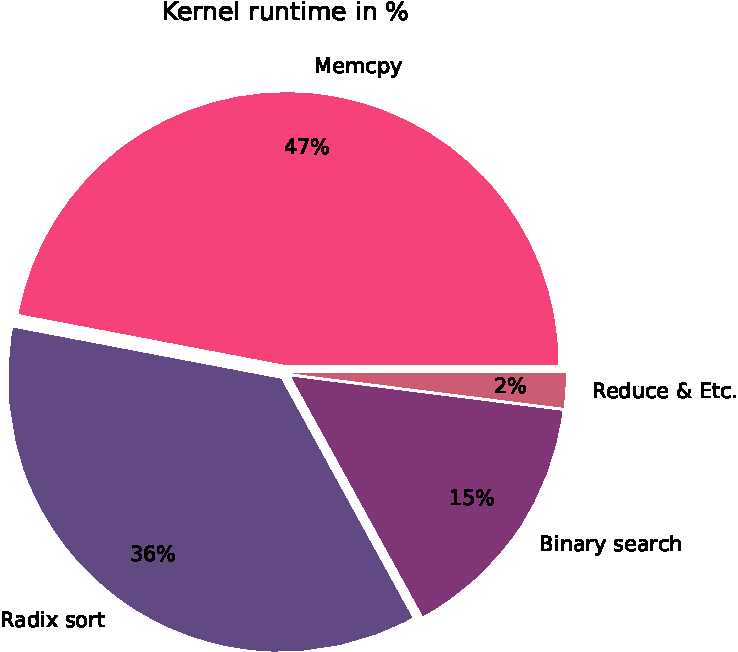
\includegraphics[width=0.8\linewidth]{figures/pdfresizer.com-pdf-crop.pdf}
\end{minipage}
\caption{Resources utilization and runtime}
    \label{fig:SMperf}
\end{figure}

For the latter, optimizations are hard to automate and perform in general.
% , as already mentioned, e.g., for fusion that includes index arithmetic. 
% The runtime of graph kernels is dependent on the input data, so in a multiple iterations algorithm, it might be profitable to fuse two kernels in one iteration and two different kernels in a different iteration. 
Kernels are compelled to satisfy certain restrictions to be fuseable: the absence of intermediate synchronization, same data access pattern, and enough resources on the device to execute the fused kernel. 
% Once again, \texttt{map/reduce} kernels could be successfully fused, but it is unclear whether GraphBLAS standard could be solely implemented in \texttt{map/reduce} terms. 
For specialization, it is better for the underlying hardware to be \emph{MIMD} for the workers to be completely independent, however GPU's architecture is \emph{SIMD}, which prevents successful specialization in many cases.

% TODO тут вывод, пока не знаю какой :)
% \subsection{Hardware implementations}

Eventually, some application-specific integrated circuits were designed to address the issues mentioned above, that basically provide hardware units for sparse matrix-matrix or matrix-vector multiplication~\cite{Song_2016, CPU-FPGA, zhang2020sparch,Systolic}. 
A brief overview could be found in~\cite{zhang2020sparch}. The implementation from~\cite{zhang2020sparch} greatly outperforms CPUs (Intel MKL\footnote{Intel MKL library: \url{https://software.intel.com/content/www/us/en/develop/tools/oneapi/components/onemkl.html}  (online; accessed:
2022-06-07)}) and GPUs (cuSPARSE\footnote{\url{https://developer.nvidia.com/cusparse} (online; accessed:
2022-06-07)}) solutions in terms of speed and power consumption. Despite high performance, such solutions do not yet provide a complete implementation of GraphBLAS (or even a subset required for a concise breadth-first search) and seem too self-contained to split the operation into phases that could be optimized in the discussed sense. However, considering high performance, it is promising to combine software and hardware parts to achieve both performance and expected usability inherent to GraphBLAS implementations.

% A notable challenge for sparse application-specific accelerators are the memory accesses. In such devices (it is also true for all devices in general) the performance, e.g. operations-per-second, are limited by the power consumption, so in order to achieve higher performance it is needed to reduce the power per operation. Memory accesses have the highest power-per-operation level in the instruction pipeline, so much of the efforts should be aimed at increasing memory access locality and cache-design as well as at reducing the number of such accesses. \todo{либо убрать, либо как-то аккуратнее сказать}

\begin{figure}[t]
    \centering
    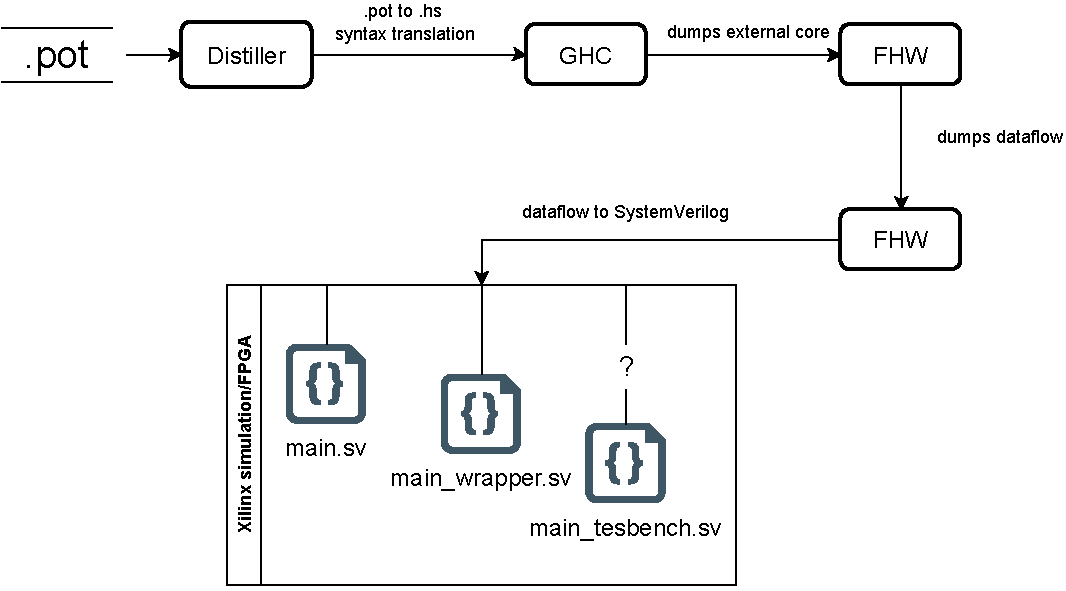
\includegraphics[width=0.9\textwidth]{figures/arch.drawio (4).pdf}
    \caption{Solution's data flow}
    \label{fig:archI}
\end{figure}

\subsection{Proposed solution}\label{sec:requirements}

To address the mentioned challenges and support automatic fusion for sparse applications, the work opts for distillation to provide fusion and high-level synthesis (HLS) to generate application-specific hardware. The first option provides low-level automatic fusion for functional programs while still making it possible to eventually use rewrite rules and staged compilation\footnote{It is noted to justify the design choice and is not the purpose of the work.}. The latter one takes into account all the software optimizations made to generate application-specific hardware, and hence it is more flexible than, e.g., hardcoded solutions for matrix multiplication.

Since distillation provides fusion for functional programs, it is left to perform HLS for a functional program. 
Modern HLS tools are imperative and do not handle arbitrary recursion. This work uses and refines the experimental compiler \emph{FHW} from~\cite{funcHLS}. 
This compiler compiles an arbitrary Haskell program into SystemVerilog utilizing parallel and pipelined dataflow intermediate representation, which allows to perform syntax-directed translation into hardware.

% is abstracted over memory operations and thus custom memory implementation could be plugged in into the backend.

The flow of data in our solution could be seen in figure~\ref{fig:archI}. We write a program that contains sparse linear algebra routines in a simple, functional language \texttt{.pot}, which is a source language for the distiller. After distillation, the transformed program is emitted into Haskell and GHC dumps the \textit{external core} representation of it. This representation is input for FHW. First, a program in external core representation is transformed into dataflow intermediate representation by using auxiliary syntax transformations. Then a program in dataflow representation is fed into FHW again to finally get SystemVerilog code in \texttt{main.sv}. Some auxiliary modules are also generated: \texttt{main\_wrapper.sv} is needed to pass arguments to \texttt{main.sv} and \texttt{main\_testbench.sv} is simulation testbench, \texttt{main\_testbench.sv} is not used for synthesis and thus is marked by \texttt{?}.

% Given the performance bottlenecks, the expected expressive power, and optimizations the following requirements could be formulated. 
% \begin{enumerate}
%     \item The software part should be expressive enough to at least define several algorithms, e.g. described in ~\cite{yang2020graphblast}
%     \item The optimizations, specified in~\ref{graphblas}, should be easily performed with the software.
%     \item The hardware should define application-specific memory system.
%     \item The hardware should be general enough to allow optimizations to be performed at software level.
% \end{enumerate}

\subsection{Distillation}

Distillation is an extension of positive supercompilation, described in~\cite{distillation}. It is a functional programs transformation technique that aims to reduce the number of required reductions and intermediate data structures. In doing so, it drives the program with the help of normal order reduction rules constructing a process graph. The process of driving could be potentially infinite, but it is bounded by homeomorphic embedding relation, which guarantees the termination of such driving. Such a finite process graph describes all possible execution paths of a program. Driving makes a transitive closure of such graph and propagates information, thus the number of required computations is reduced: transitive closure removes intermediate nodes, and information propagation makes extra case expressions unnecessary. An example of such transformation could be seen below, where a sequence of \texttt{append} functions is transformed to iterate over each list only once. 

% caption={Program before transformation}
% \begin{minipage}[t]{0.3\textwidth}
%     \begin{lstlisting}[language=Haskell] 
% append (append xs ys) zs where

%   append xs ys = case xs of
%     [] -> ys
%     (x:xs') -> x : (append xs' ys)
% \end{lstlisting}
% \vfill
% \captionof{listing}{Program before transformation}
% \end{minipage}
% \hfill
% \begin{minipage}[t]{0.3\textwidth}
%         \centering
%         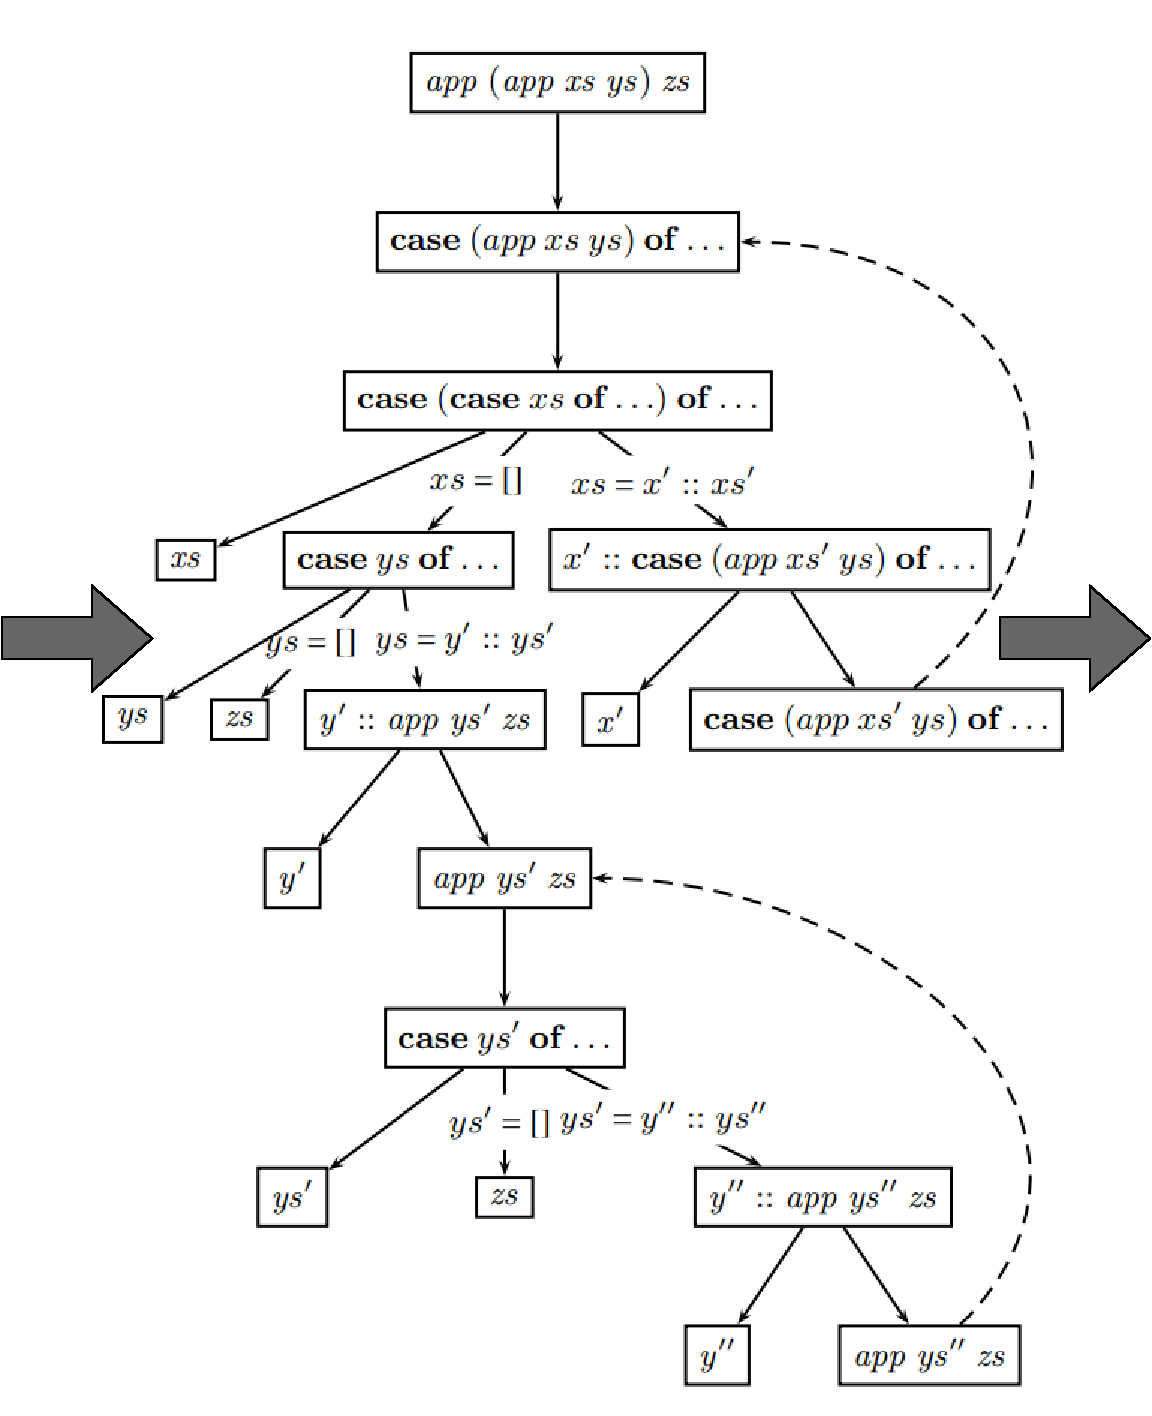
\includegraphics[width=\textwidth]{figures/test.drawio.pdf}
%         \captionof{figure}{Process graph}
%         % \caption{Process graph}
% \end{minipage}
% \hfill
% \begin{minipage}[t]{0.3\textwidth}
%     \begin{lstlisting}[language=Haskell]
% f xs ys zs where

%  f xs ys zs = case xs of
%     [] -> case ys of
%       [] -> zs
%       y':ys' -> y': (g ys') where
          
%          g ys = case ys of
%             [] -> zs
%             y':ys' -> y':(g ys')
%     x':xs' -> x':(f xs' ys zs)
% \end{lstlisting}
% \captionof{listing}{Program after transformation}
% \end{minipage}

\begin{figure}[t]
\begin{tabular}{@{}m{0.33\linewidth}m{0.33\linewidth}m{0.33\linewidth}}
 \begin{minipage}[t]{0.33\textwidth}
 \begin{minted}[fontsize=\scriptsize]{Haskell}
  append (append xs ys) zs where
  
   append xs ys = case xs of
    [] -> ys
    (x:xs') -> x : (append xs' ys)
  \end{minted}
% \captionof{listing}{Program before transformation}
\end{minipage}&
\begin{minipage}[t]{0.33\textwidth}
    {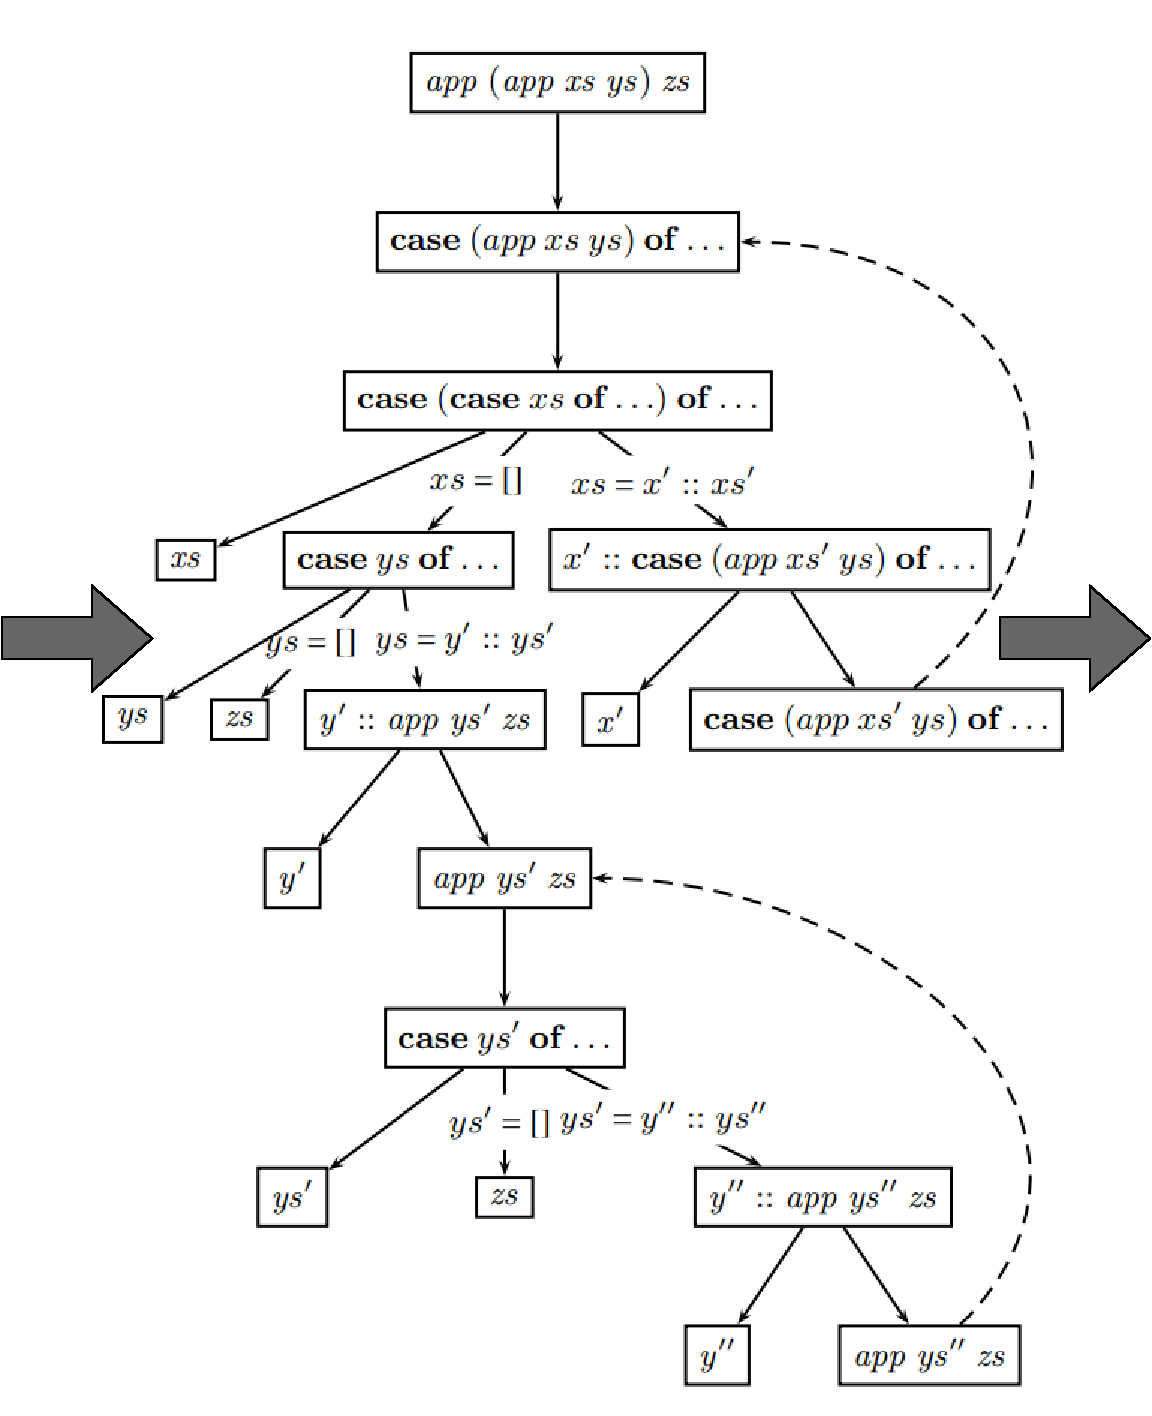
\includegraphics[width=1\linewidth]{figures/test.drawio.pdf}}
% \captionof{figure}{Process graph}
\end{minipage}
&
\begin{minipage}[t]{0.33\textwidth}
\begin{minted}[fontsize=\scriptsize]{Haskell}
f xs ys zs where

 f xs ys zs = case xs of
    [] -> case ys of
      [] -> zs
      (y':ys') -> y' : (g ys') where
          
         g ys = case ys of
            [] -> zs
            (y':ys') -> y' : (g ys')
    (x':xs') -> x' : (f xs' ys zs)
\end{minted}
% \captionof{listing}{Program after transformation}
\end{minipage}
\\
\begin{minipage}[t]{0.33\textwidth}
\captionof{listing}{Program before transformation}
\end{minipage} &
\begin{minipage}[t]{0.33\textwidth}
\captionof{figure}{Process graph}
\end{minipage} &
\begin{minipage}[t]{0.33\textwidth}
\captionof{listing}{Program after transformation}
\end{minipage}
% \captionof{listing}{Program before transformation}&
% \caption{{\fontfamily{pcr}\selectfont spy} Plot of 4-bus Test System}\label{fig:Image_34}&
% \captionof{listing}{Program before transformation}\\
\end{tabular}
\end{figure}

The process graph in the middle is obtained from driving the program to the left and the right program is residualized from the process graph. Dashed edges lead to recursive function calls, but before the call information is propagated.

\subsection{FHW}

FHW~\cite{funcHLS} is a compiler that compiles a Haskell program into SystemVerilog. Notably, the tool is purely functional and allows programs with arbitrary recursion. The compiler relies on specific syntax transformations, which make eventual translation into hardware easier. The most crucial transformations are \textit{defunctionalization}, which encodes higher order functions, making them possible to be represented in hardware; \textit{continuation-passing-style} (CPS) transformation, which makes control flow explicit by passing it via additional arguments to functions; and encoding recursive types with explicit pointers. CPS makes each recursive function tail-recursive, hence there is no need to maintain a stack for each function call: each group of mutually recursive functions shares the same heap, which stores their continuations. This makes it easier to return values to the caller.

\begin{table}[t]
\footnotesize
\centering
\begin{tabular}{ |l|l|} 
\hline
\rowcolor{LightBlue}
{Actor} & {Description}\\
\hline
\multirow{2}{0.2\linewidth}{\texttt{primitive}} & \multirow{2}{0.5\linewidth}{Performs built-in operations, e.g., integer addition or constructor application.}\\
{} & {}\\
\hline
\multirow{2}{0.15\linewidth}{\texttt{destruct}} & \multirow{2}{0.5\linewidth}{Disassembles a value of algebraic data type. It has an output per each data type's constructor field.}\\
{} & {} \\
\hline
\multirow{2}{0.15\linewidth}{\texttt{fork}} & \multirow{2}{0.5\linewidth}{Consumes a single input token and copies it to each of its
output channels.}\\
{} & {} \\
\hline
\multirow{2}{0.15\linewidth}{\texttt{demux}} & \multirow{2}{0.5\linewidth}{Behaves like a demultiplexer, i.e. routes the value input to the channel chosen by the choice input.}\\
{} & {}\\
\hline
\multirow{3}{0.15\linewidth}{\texttt{mux}} & \multirow{3}{0.5\linewidth}{Behaves like a multiplexer, i.e. chooses the value from inputs according to the choice input and routes it to the output.} \\
{} & {}\\
{} & {}\\
\hline
\multirow{2}{0.15\linewidth}{\texttt{read}} & \multirow{2}{0.5\linewidth}{Constructs a pointer from a value.} \\
{} & {}\\
\hline
\multirow{2}{0.15\linewidth}{\texttt{write}} & \multirow{2}{0.5\linewidth}{Returns a value for a pointer.} \\
{} & {}\\
\hline
\multirow{2}{0.15\linewidth}{\texttt{merge}} & \multirow{2}{0.5\linewidth}{It chooses an available token from one of its inputs and routes it to its output.} \\
{} & {}\\
\hline
\multirow{2}{0.15\linewidth}{\texttt{mergeChoice}} & \multirow{2}{0.5\linewidth}{Same as above but also generates a token
indicating which input channel provided the selected token.}\\
{} & {}\\
\hline
\multirow{2}{0.15\linewidth}{\texttt{source}} & \multirow{2}{0.5\linewidth}{Serves as an entry point to dataflow network, it is allowed to have no inputs.}\\
{} & {}\\
\hline
\multirow{2}{0.15\linewidth}{\texttt{sink}} & \multirow{2}{0.5\linewidth}{Serves as an output of dataflow network, it is allowed to have no outputs.}\\
{} & {}\\
\hline
\end{tabular}
    \caption{FHW actors}
    \label{tab:actors}
\end{table}


The compiler relies on dataflow intermediate representation that is constructed from combinations of predefined basis actors. Then, such actors are implemented in SystemVerilog and cooperate via valid/ready protocol. Each actor is required to have at least one input and one output, thus a special \texttt{Go} token is added to trigger dataflow execution and constants creation. The available actors are summarized in table~\ref{tab:actors}.

Each function and recursive data type has its own heap, which increases parallelism, but maintaining equally-sized memory spaces could be quite expensive. Memory at the moment is implemented as \texttt{bram} blocks in hardware. The memory is assumed to be garbage collected, but garbage collector is not implemented. To break cycles in valid/ready networks additional buffers are inserted.

